\chapter{Solution Design: Improved Kepler Visualisation Tool}\label{C:sd}

This section discusses the design of the deliverable visualisation, The Improved Kepler Visualisation Tool(IKVT) that was created for this project. It details the key design decisions revolving around structure, asthetics, and functionality that were made about the visualisation. 
% Description of tool
To help users to understand more about the planets outside of our solarsystem, this project aims to improve an existing visualisation, The Kepler Visualisation Tool that was discussed in the previous chapter, which whist displaying exoplanets and some of thier features, it lacks interactivity for users trying to use it to help comprehend the ...~. The IKVT expands on the preexisting Kepler Visualisation Tool by adding key elements of interativity that are missing with the existing visualisation.

To aid in the comprehesion of exoplanets and their information contained in the ...~ dataset, IKVT 
% Aim of the visualisation ~

% Basic functionality of the visualisation - massive

% How visualisation represents each component

% Does it satisfy each requirements

% Discuss the features of other viusalisations incorporated

\section{System design and structure}
BASIC Class structure

Data structure

UML CLass Diagram

Sequence Diagram

\section{Design Features}
\subsection{Main interface components}
The visualisation was designed to emphasis small multiples and filtering of the Exoplanets to display the information more clearly to users. 
\\\\
Instead of the visualisation only answering the 5 key questions as proposed in the proposal, the aim will now be displaying as much of the information in the dataset as possible without detracting from the effectiveness of the visualisation whilst still answering the questions. 
\\\\
This is because the 5 questions did not fully utilize the information in the dataset. 
\\\\
However I will need to ensure the effectiveness of the visualisation does not become diminished by trying to convey to much information which would lead to cluttering and overlapping in the visualisation, as well as information overload for users. There will also be larger emphasis placed on making the existing system more usable by improving the interaction methods for users. The following list outlines the new requirements for the visualisation being developed. This will be done by providing GUI elements for each form of interaction with the system, as well as ensuring all interaction methods are intuitive for users. 
\subsubsection{Spacial arrangement of components}
As the majority of the interaction and movement of visualisation elements occurs in the center of the window it caused a aspect ratio that was not suitable . It was BETTER~ to use 2 vertical columns to view and control the visualisation as it had a higher aspect ratio which allowed more of the content to be seen on the screen at once thanks to the fact that the majority of computer screens have a wide ratio.

\begin{figure}[h!]
  \centering
      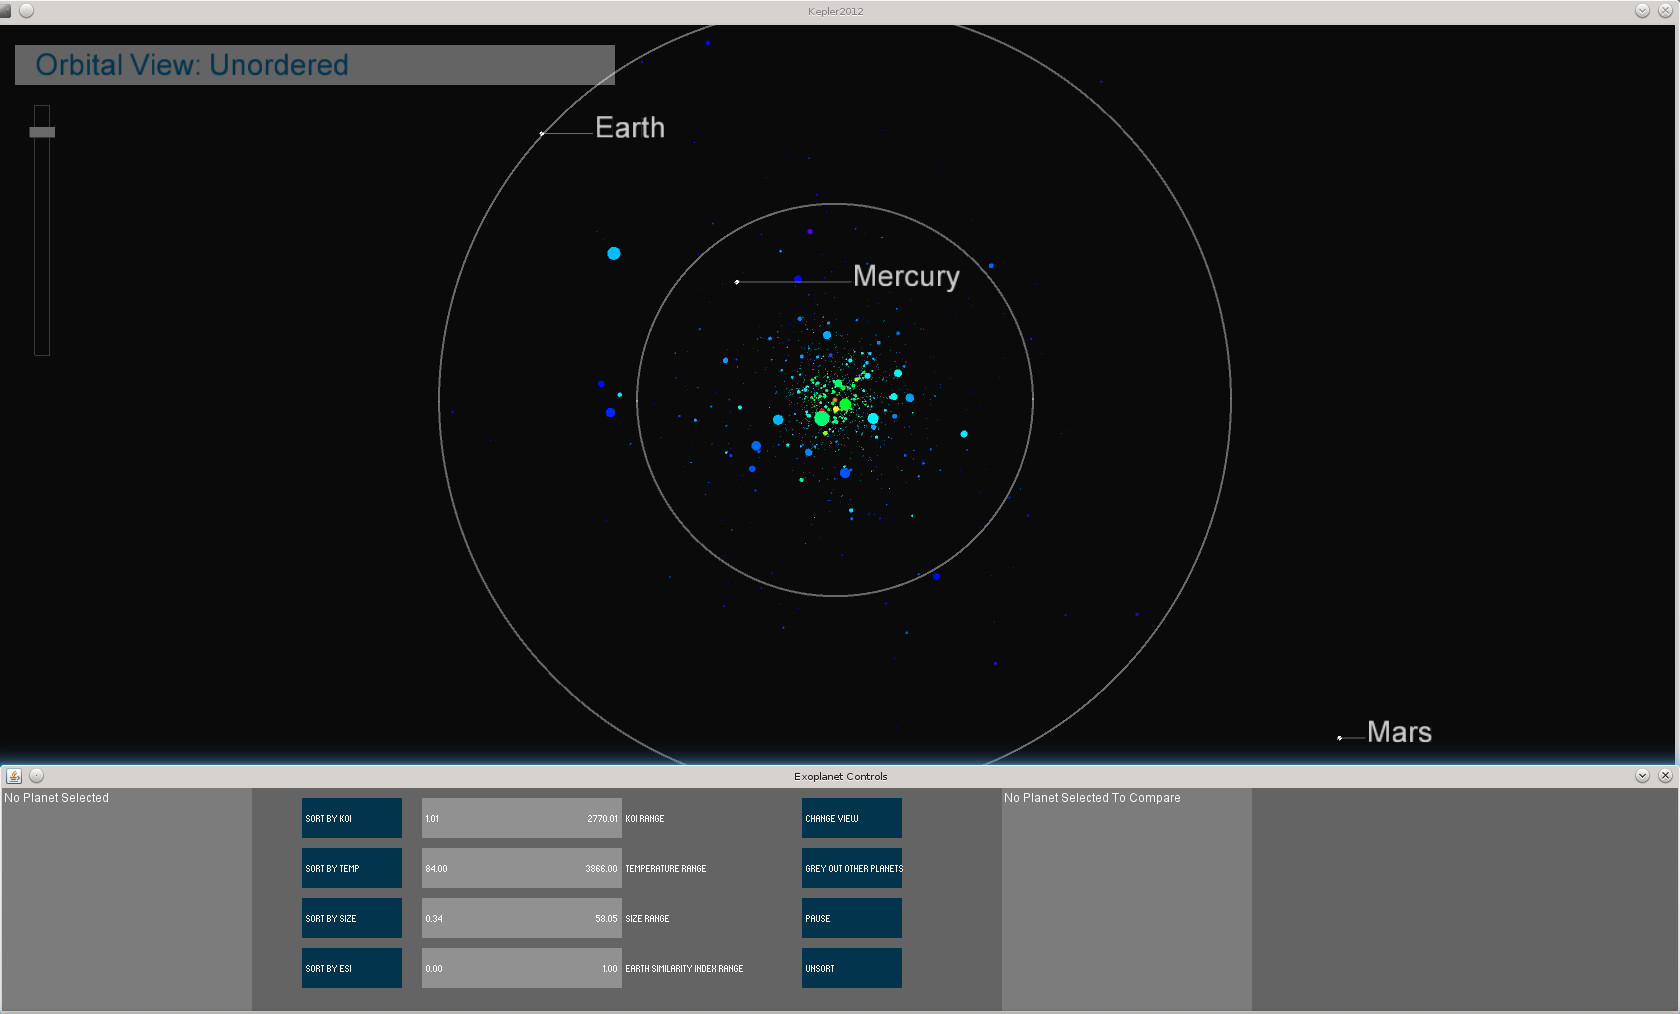
\includegraphics[width=0.8\textwidth]{images/layout_horizontal.jpg}
  \caption{Original Horizontal Layout}  
        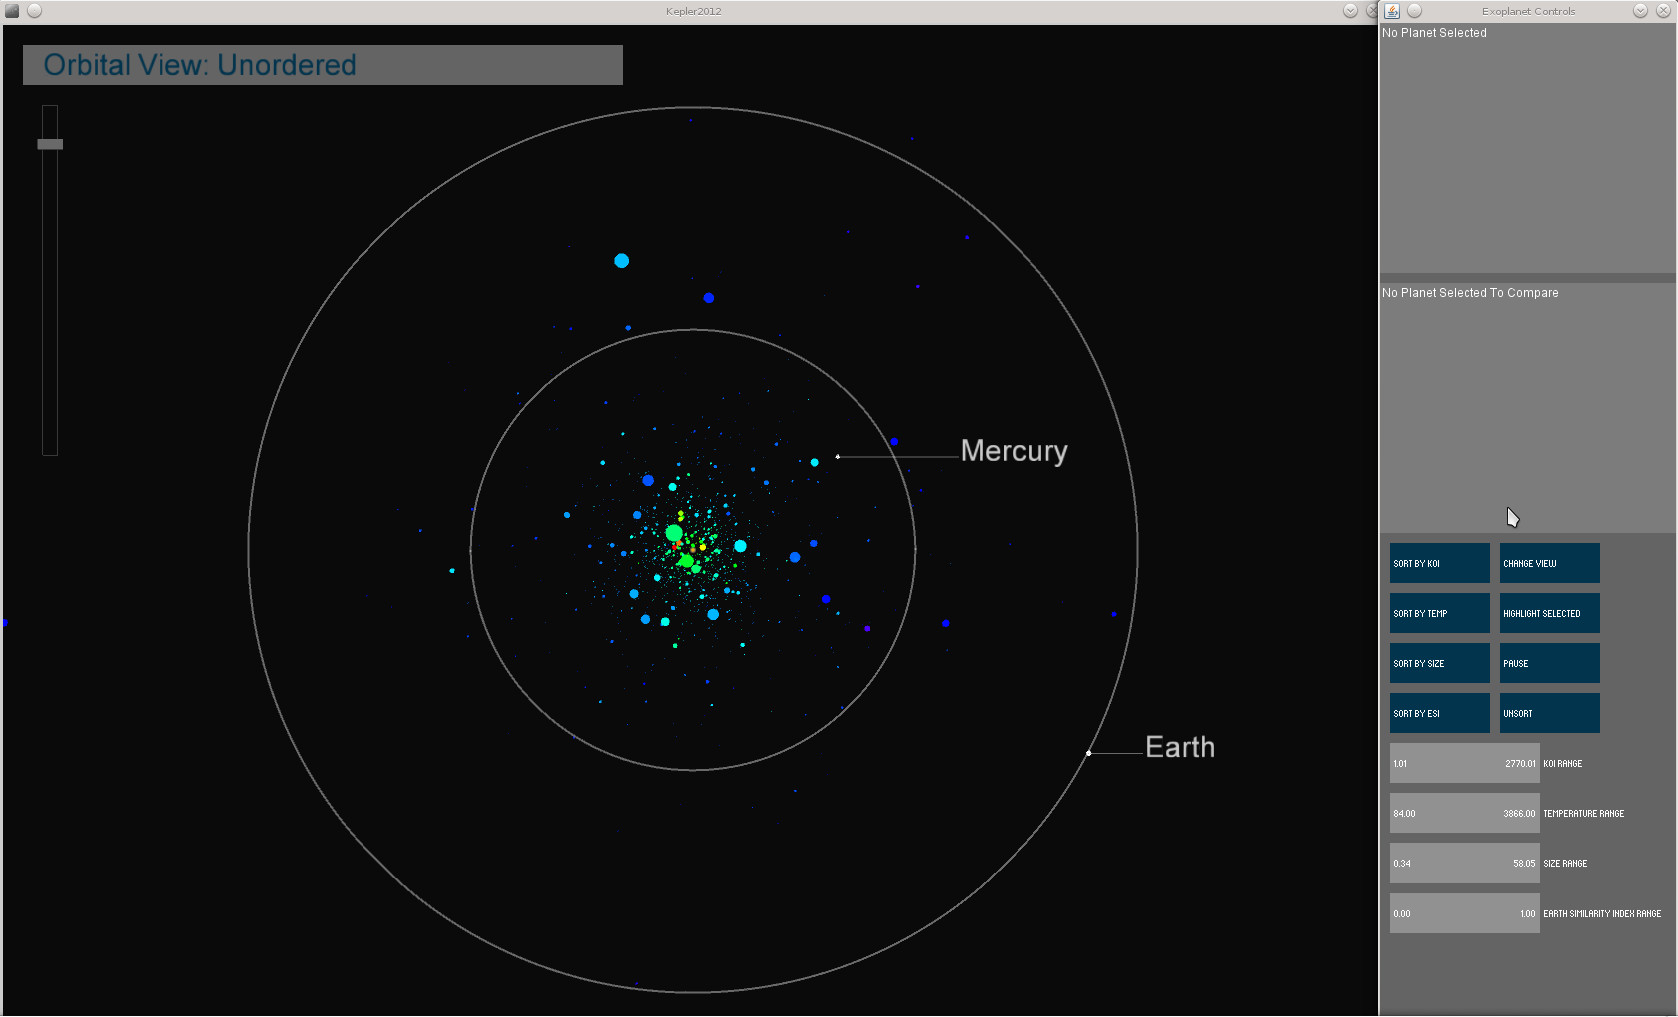
\includegraphics[width=0.8\textwidth]{images/layout_vertical.jpg}
  \caption{Improved Vertical Layout}
\end{figure}

\subsubsection{Navigation Window(BETTER TITLE~)}
Description of navigation window

Description of each button

Description of each slider

Description of text boxes

Due to the need for increased user interaction with the visualisation a window is required to house the buttons, range selectors, and text areas. These elements are needed as the different methods that users can use to interact with the visualistaion need to be visually apparent to ensure that the system can be easily used without prior experience. A way to do this is to provide clearly labelled interactive elements and tooltips explaining what they do.((REFERENCE))~. These tooltips are widely used as a method of informing a user about the purpose of an item by hovering over it. This removes the need to click on a button to discover its effect.

\subsubsection{Visualisation Layout for Kinect sensor}
As the Kinect sensor no longer requires the use of a mouse the visualisation design needs to be modified to accomodate the use of gestures. For this project this meant incorporating new cursers to indicate the state of the visualisation. There are 7 states that the curser needs to be able to be in to inform the user of what action they are performing. These states are

\begin{enumerate}
 \item default curser, hand is at rest
 \item panning up, hand is raised
 \item panning down, hand is lowered
 \item panning left, hand is to the left
 \item panning right, hand is to the right
 \item zooming in, hand is pressed forward
 \item zooming out, hand is pulled backwards
\end{enumerate}

Having a range of icons that clearly display these states is vital for keeping the user informed of what they are doing. The icons designed for this purpose are in the following figure

\begin{figure}[h!]
  \centering
  ~
      %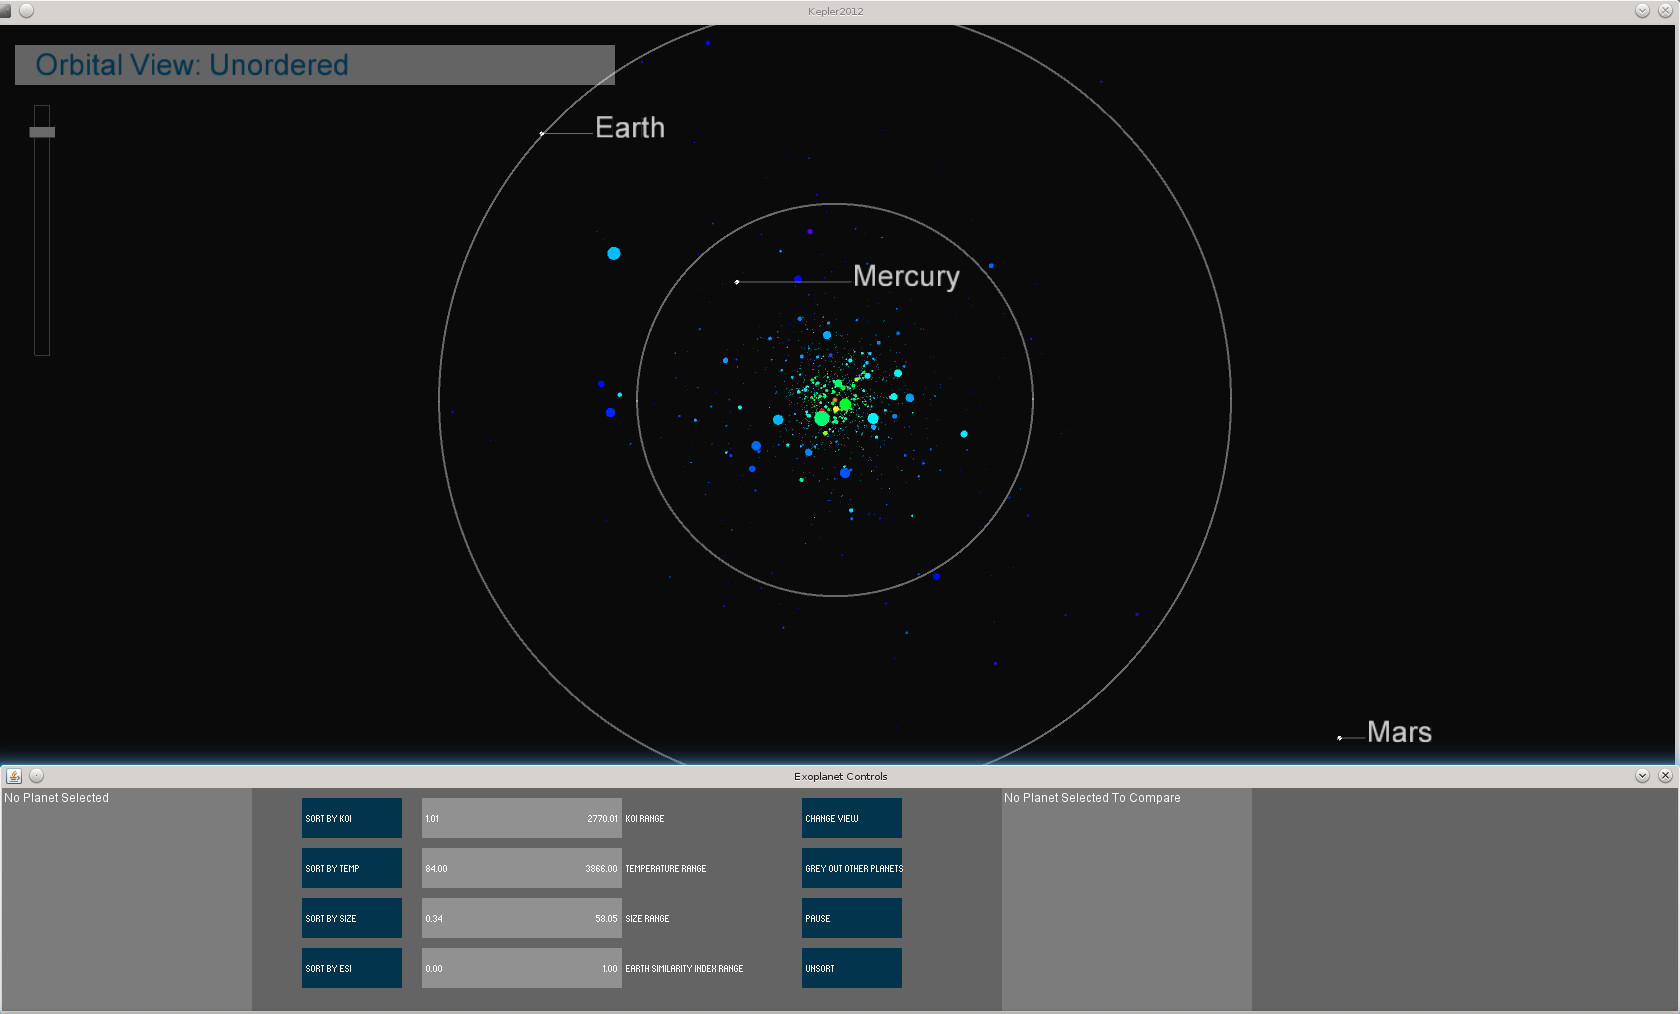
\includegraphics[width=0.8\textwidth]{images/layout_horizontal.jpg}
  \caption{Cursers for Kinect sensor}  
\end{figure}

In addition to this, the screen needs to display the user in relation to the screen, an effective way to do this is to display a washed out representation of themselves in the background of the visualisation. 